\documentclass[border=4pt,12pt]{standalone}
% House style for redrawn exam diagrams (diagram-v4: 0.4pt lines, filled -latex arrows, fine dashes; stipple and hatching drawn as real dots/lines (no PDF/SVG patterns, so they render in every browser and at any scale); transparent background). Every figure \input's this.
\usepackage{amsmath,amssymb}
\usepackage{txfonts}
\usepackage{pdfrender,xcolor}
% \halo{text}: label on shading. The shading stops just around each letter's outline (a thin knock-out that follows the
% glyphs, like the papers' typesetting), never a box. Owner: "I don't want a box around the text".
\newcommand{\halo}[1]{\leavevmode\rlap{\pdfrender{TextRenderingMode=2,LineWidth=2.2pt,LineJoinStyle=1,StrokeColor=white,FillColor=white}#1}#1}
\usepackage{tikz,pgfplots}
\pgfplotsset{compat=1.18}
\usetikzlibrary{arrows.meta,calc,angles,quotes,patterns,patterns.meta,intersections,positioning,decorations.markings,shapes.geometric}
% Stipple and hatching are drawn as actual dots / lines clipped to the region (path picture), NOT as pattern fills:
% SVG <pattern> fills vanish or blur when browsers scale the image, so the owner could not see the shading.
% Each dot is a 0.72pt square (keeps SVGs small; reads as a dot at print size). Dots sit on one global staggered grid, so neighbouring regions line up.
\makeatletter
\newdimen\ex@x \newdimen\ex@y \newdimen\ex@xa \newdimen\ex@ya \newdimen\ex@xb \newdimen\ex@yb \newcount\ex@row
\def\exam@stipplecolor{black!75}\def\exam@dotr{0.42pt}\def\exam@dotgap{2.5}
\def\ex@rowdots{\ifdim\ex@x<\ex@xb \pgfpathrectangle{\pgfqpoint{\dimexpr\ex@x-0.36pt\relax}{\dimexpr\ex@y-0.36pt\relax}}{\pgfqpoint{0.72pt}{0.72pt}}\advance\ex@x by \exam@dotgap pt\relax\expandafter\ex@rowdots\fi}
\def\exam@stipple{%
  \pgftransformreset% dots are sized in real points even inside scaled pictures
  \pgfpointanchor{path picture bounding box}{south west}\ex@xa=\pgf@x \ex@ya=\pgf@y
  \pgfpointanchor{path picture bounding box}{north east}\ex@xb=\pgf@x \ex@yb=\pgf@y
  \pgfsetfillcolor{\exam@stipplecolor}\pgfmathsetmacro\ex@h{\exam@dotgap/2}%
  \pgfmathtruncatemacro\ex@r{floor(\ex@ya/\ex@h)-1}\ex@row=\ex@r\relax
  \ex@y=\ex@r\dimexpr\ex@h pt\relax
  \loop\ifdim\ex@y<\ex@yb
    \pgfmathtruncatemacro\ex@c{floor(\ex@xa/\exam@dotgap)-1}\ex@x=\ex@c\dimexpr\exam@dotgap pt\relax
    \ifodd\ex@row \advance\ex@x by \ex@h pt\fi
    \ex@rowdots
    \advance\ex@y by \ex@h pt \advance\ex@row by 1
    \ifnum\numexpr\ex@row-(\ex@row/4)*4\relax=0 \pgfusepath{fill}\fi% flush every 4 rows: bounded TeX memory, few clip copies in the SVG
  \repeat\pgfusepath{fill}}
\newdimen\ex@d
\def\exam@hatch#1{% #1 = 1 for /, -1 for \ ; lines 45 degrees, 3pt apart
  \pgftransformreset
  \pgfpointanchor{path picture bounding box}{south west}\ex@xa=\pgf@x \ex@ya=\pgf@y
  \pgfpointanchor{path picture bounding box}{north east}\ex@xb=\pgf@x \ex@yb=\pgf@y
  \ex@d=\dimexpr\ex@yb-\ex@ya\relax \ex@x=\dimexpr\ex@xa-\ex@d\relax
  \loop\ifdim\ex@x<\ex@xb
    \ifnum#1>0 \pgfpathmoveto{\pgfqpoint{\ex@x}{\ex@ya}}\pgfpathlineto{\pgfqpoint{\dimexpr\ex@x+\ex@d\relax}{\ex@yb}}%
    \else \pgfpathmoveto{\pgfqpoint{\ex@x}{\ex@yb}}\pgfpathlineto{\pgfqpoint{\dimexpr\ex@x+\ex@d\relax}{\ex@ya}}\fi
    \advance\ex@x by 4.24pt
  \repeat
  \pgfsetlinewidth{0.4pt}\pgfsetstrokecolor{black}\pgfusepath{stroke}}
\def\examstipple{\exam@stipple}\def\examhatch{\exam@hatch}\def\examsetstipplecolor#1{\def\exam@stipplecolor{#1}}\def\examsetdotgap#1{\def\exam@dotgap{#1}}
\makeatother
% (legacy pattern kept for old files)
% staggered stipple like the NESA papers' dotted shading
\pgfdeclarepatternformonly{exam stipple}{\pgfpointorigin}{\pgfqpoint{2.2pt}{2.2pt}}{\pgfqpoint{2.2pt}{2.2pt}}{%
  \pgfpathcircle{\pgfqpoint{0.55pt}{0.55pt}}{0.42pt}\pgfpathcircle{\pgfqpoint{1.65pt}{1.65pt}}{0.42pt}\pgfusepath{fill}}
\tikzset{
  every picture/.style={line width=0.6pt, >={Latex[length=2mm,width=1.3mm]}},
  curve/.style={line width=0.6pt},
  open arrow/.style={-{Latex[length=2mm,width=1.3mm]}},  % owner: filled -latex heads everywhere, no open chevrons
  aux/.style={dash pattern=on 2pt off 1.5pt, line width=0.6pt},
  shade/.code={\def\exA{#1}\def\exB{none}\ifx\exA\exB\else\pgfkeysalso{fill=black!18}\fi},
  shade/.default=on,
  shade dots/.style={fill=none, path picture={\examstipple}},
  stipple color/.code={\examsetstipplecolor{#1}},
  stipple gap/.code={\examsetdotgap{#1}},
  shade dense dots/.style={fill=none, stipple gap=1.6, path picture={\examstipple}},
  shade hatch/.style={fill=none, path picture={\examhatch{1}}},
  shade hatch reverse/.style={fill=none, path picture={\examhatch{-1}}},
  shade solid/.style={fill=black},
  pt/.style={circle, fill, inner sep=1.1pt},
  open pt/.style={circle, draw, fill=white, inner sep=1.1pt},
}
\pgfplotsset{
  exam axes/.style={axis lines=middle, axis line style={->}, xlabel={$x$}, ylabel={$y$},
    xlabel style={anchor=west}, ylabel style={anchor=south}, tick label style={font=\small},
    every axis plot/.append style={line width=0.6pt, black}, samples=200, clip=false,
    enlargelimits=false, axis on top},
}

\begin{document}
% 2025 Penrith AT4 Q24 solution: y=ln x, rectangle [0,e^2]x[0,a], regions A (light) and B (darker), trapezia with two strips of width h (crop pixels, y down)
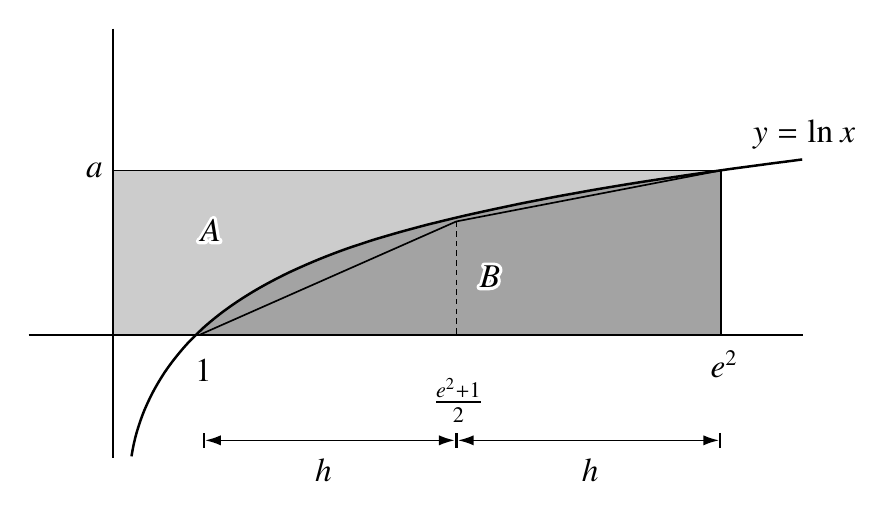
\begin{tikzpicture}[x=0.0127cm,y=-0.0127cm,font=\fontsize{12}{14}\selectfont]
  \fill[black!20] (84.5,152) rectangle (692.5,316.5);
  \fill[black!36] (171,316.5) -- plot[smooth] coordinates {(172,310) (179,304.5) (186.2,299.2) (193.3,294.2) (200.7,289.1) (208.1,284.3) (215.6,279.5) (223.3,274.9) (231,270.5) (238.7,266.1) (246.7,261.9) (254.7,257.8) (262.8,253.9) (271,250) (279.2,246.3) (287.5,242.8) (295.9,239.2) (304.3,235.9) (312.9,232.6) (321.5,229.5) (330.1,226.4) (338.8,223.5) (347.6,220.6) (356.4,217.9) (365.2,215.2) (374.1,212.6) (383,210.1) (392.1,207.6) (401.1,205.3) (410.2,203) (419.3,200.7) (428.4,198.5) (437.6,196.4) (446.8,194.3) (456,192.3) (465.3,190.3) (474.5,188.4) (483.8,186.5) (493.1,184.7) (502.5,182.9) (511.8,181.1) (521.2,179.4) (530.6,177.7) (539.9,176.1) (549.3,174.5) (558.8,172.8) (568.2,171.3) (577.7,169.7) (587.1,168.2) (596.6,166.7) (606.1,165.2) (615.6,163.7) (625.1,162.2) (634.6,160.8) (644.1,159.3) (653.7,157.8) (663.3,156.4) (672.8,154.9) (682.4,153.5) (692,152)} -- (692.5,316.5) -- cycle;
  \draw (0,316.5) -- (775,316.5);
  \draw (84.5,10) -- (84.5,440);
  \draw (84.5,152) -- (692.5,152) -- (692.5,316.5);
  \draw[line width=0.9pt] plot[smooth] coordinates {(103,438) (105.1,426.7) (107.8,415.6) (111.2,404.6) (115.1,393.9) (119.6,383.6) (124.8,373.1) (130.4,363.2) (136.6,353.4) (143.4,343.9) (150.7,334.7) (158.4,325.8) (166.6,317.4) (175.3,309.1) (184.4,301.3) (193.8,293.9) (203.9,286.6) (214.1,279.8) (224.9,273.1) (235.9,266.8) (247.1,260.8) (258.8,254.9) (270.5,249.5) (282.6,244.2) (294.7,239.2) (307.1,234.4) (319.7,229.8) (332.3,225.6) (345.1,221.4) (358.2,217.5) (371.3,213.7) (384.5,210.1) (398,206.5) (411.4,203.2) (424.9,199.9) (438.6,196.7) (452.1,193.7) (465.9,190.7) (479.6,187.8) (493.4,184.9) (507.3,182.2) (521.1,179.5) (534.9,176.9) (548.9,174.4) (562.7,171.9) (576.7,169.5) (590.5,167.2) (604.6,164.9) (618.6,162.7) (632.5,160.6) (646.6,158.5) (660.7,156.4) (674.8,154.4) (688.9,152.4) (703,150.4) (717.1,148.5) (731.4,146.6) (745.5,144.7) (759.7,142.9) (774,141)};
  % trapezia (solution additions)
  \draw (171,316.5) -- (428,203) -- (692.5,152);
  \draw[aux] (428,203) -- (428,316.5);
  \draw[|<->|] (175,422) -- (428,422);
  \draw[|<->|] (428,422) -- (692.5,422);
  \node at (295,452) {$h$};
  \node at (562,452) {$h$};
  \node at (430,382) {$\frac{e^2+1}{2}$};
  \node at (175,352) {$1$};
  \node at (696,346) {$e^2$};
  \node at (66,152) {$a$};
  \node at (182,212) {\halo{$A$}};
  \node at (461,258) {\halo{$B$}};
  \node at (776,116) {$y=\ln x$};
\end{tikzpicture}
\end{document}
